\documentclass[12pt]{article}

\usepackage[utf8]{inputenc}
\usepackage[bulgarian]{babel}
\usepackage{graphicx}
\usepackage{sidecap}  %required for side captions
\usepackage{amssymb}
\usepackage{amsmath}
\usepackage{hyperref}
\usepackage{commath}  
\usepackage[top=1.3in, bottom=1.5in, left=1.3in, right=1.3in]{geometry}


\begin{document}
	\begin{center}
        \LARGE{\textbf{Тема: Разширяване на проект по Уеб технологии - Презентации по Web(календар) с AWS EC2, AWS RDS, AWS CodeCommit}}
        
        \bigskip
        \Large{Предмет: Приложно-програмни интерфейси за работа с облачни архитектури с Амазон Уеб Услуги(AWS)}
        
        \medskip
        \Large{Изготвил: Дияна Йорданова, фн: 81547, имейл: dijanaj@uni-sofia.bg}
        
        \medskip
        \Large{Лектор: доц. д-р Милен Петров, година: 2020}
        
        \bigskip
	\end{center}
    
    
  %  \newpage
    \tableofcontents
    \bigskip
    \bigskip
    \newpage
  
\section{Условие} 

\noindent Разширяване на съществуващ проект по Уеб технологии с поне една услуга на AWS. Tex документация на разширения проект и диаграми, изобразяващи кратко ръководство за потребителя.   
\medskip


\noindent \textbf{Условие на разширения проект:} 
\noindent Уеб приложението подпомага организацията за представяне на презентации, по предмета Web технологии, от студенти. В системата е изградена функционалност за регистриране и вход на студенти. При вход в системата всеки студент трябва да въведе своя факултетен номер и парола. С тази функционалност всеки студент има права да редактира календара като избере час и дата, които са свободни. Ако няма регистриран студент, то неговите права са ограничени – той има права само да преглежда календара и информацията в него, но не и да извършва промени върху календара. Всеки регистриран потребител има възможност да запази дата за представяне на презентация. Запазването се осъществява само ако избраната дата вече не е запазена от друг студент. За всяка запазена дата от един студент има възможност за изтриване на датата и за избиране на нова такава.   
\section{Въведение}

Документацията ще представи основните идеи за създаването на проекта и неговото разширение с AWS услуги.
\medskip

\noindent Разширяването на проекта е вдъхновен от курса по Приложно-програмни интерфейси за работа с облачни архитектури с Амазон Уеб Услуги (AWS), в който бяха засегнати различни AWS услуги. За целта на проекта са използвани следните услуги:
\begin{itemize}
    \item AWS Relational Database Service (RDS)
    
    \item AWS Elastic Compute Cloud (EC2)
    
    \item AWS CodeCommit
\end{itemize}

\noindent В проекта е засегнат проблем, чието решение подпомага участниците от курса по Web технологии. В курса всяка година студентите избират теми, върху които да разработят реферат. След завършване на реферата всеки студент представя и запознава своите колеги с неговата тема. За целта се запазва определен час и ден, в който това да се осъществи. На този етап за запазване на презентации се използва споделена таблица в Google Docs. Недостатъкът при използването на таблица в Google Docs, е че всяка година трябва да се създаде нова таблица и да се въведат валидни дати и час, в които всеки студент да запише своите теми. Това затруднява работата на всички участници в курса. При въвеждане на данни от двама студенти за една дата се губят данни, което води до опасността студент да няма запазена дата за представяне на презентация. С помощта на създадената система, бързо и лесно, всеки студент може да запази дата за своята презентация. 

\section{Теория}
\noindent В този раздел ще бъдат разгледани само по-ключови решения, засягащи архитектурата на приложението и AWS услугите, използвани за разширяването му.
\medskip

\noindent За разширяването на Уеб приложението са използвани следните AWS услуги:  
\medskip

\noindent \textbf{AWS Relational Database Service (RDS):} услуга, която позволява лесно настройване, опериране и мащабиране на релационни бази данни като MariaDB, която се използва в разглеждания проект. AWS RDS се грижи за голяма част от административните задачи по поддържането на релационната база данни. Част от тези задачи са security updates, availability, data encryption, настройване на различни видове аларми и създаване на backup на базата. Това позволява на потребителя да се фокусира върху менажирането на съдържанието в базата.
\medskip

\noindent \textbf{AWS Elastic Compute Cloud (EC2):} уеб услуга, която осигурява сигурен, преоразмерим изчислителен капацитет в cloud-а чрез използване на виртуални машини. Този подход осигурява пълен контрол върху всички компютърни ресурси и позволява работа в сигурна среда на Amazon. Също така, предоставя лесна интеграция с други AWS услуги като например AWS RDS чрез Virtual Private Cloud (VPC), което е частна виртуална мрежа в cloud-а на Amazon. Ресурсите, свързани към дадена мрежа имат видимост помежду си, като контролът на достъп се осъществява чрез security group, в която се добавят дадени правила, ограничаващи достъпа. Пример за такова правило е отваряне и затваряне на дадени портове. 
\medskip

\noindent \textbf{AWS CodeCommit:} услуга, която дава възможност за управление на source code-а на приложението. Тя предоставя подсигурени хранилища за код, базирани на Git. Достъпът до тези хранилища се контролира чрез Identity Access Management (IAM). Като повечето услуги на AWS, CodeCommit лесно се интегрира с други услуги като например EC2. Това позволява бързо публикуване на променения source code. 
\medskip

%\newpage

\section{Използвани технологии}
\noindent За изграждането на web приложението са използвани следните стандартни технологии и подходи:

\begin{itemize}
\item \textbf{Frond-end}: HTML5, CSS3, JavaScript
\item \textbf{Back-end}: PHP version 'PHP 7.3.11'
\item \textbf{Database}:  MySQL (MariaDB) version '10.4.8-MariaDB'
\item \textbf{Cloud}:
\begin{itemize}
\item AWS RDS (MariaDB)
\item AWS EC2 'Amazon Linux 1 AMI 2.0.20200406.0 x86-4 HVM gp2'
\item AWS CodeCommit (Git) 
\end{itemize}
\end{itemize}

%\newpage

\section{Инсталация и настройки}
\subsection{AWS Relational Database Service}
\noindent Създава се MySQL (MariaDB) база данни с необходимата за проекта архитектура. Изпълняват се следните стъпки:
\medskip

\noindent \textbf{Security group ->}

\noindent \textbf{inbound rules ->}

\noindent \textbf{add rule ->}

\noindent \textbf{CP traffic (custom rule) with default IPs}
\medskip

\noindent Свързването към базата се осъществява с помощта на допълнителни инструменти като например MySQL Workbench. В инструмента се въвежда endpoint и порт на използваната база. Предоставят се username и password, създадени при инициализацията на базата. Import-ва се .dump файл, който създава всички таблици със съответните ограничения и въвежда всички данни, налични до този момент в тях. След успешното изпълнение на стъпките, базата данни е готова за употреба. За по-голяма сигурност AWS предоставя възможност за създаване на Snapshot на базата. Това е прост механизъм за Backup, който запазва текущото състояние на базата и при настъпил проблем позволява лесно възвръщане към предходен Snapshot.
\medskip

\subsection{AWS CodeCommit}
\noindent Създава се хранилище(AWS CodeCommit - Repository) от AWS Console. За клониране на хранилището се добавят следните git команди от фигура 1. Те синхронизират конфигурационните файлове, което дава възможност за authentication в CodeCommit. 
\medskip

\begin{figure}[h!]
\centering
    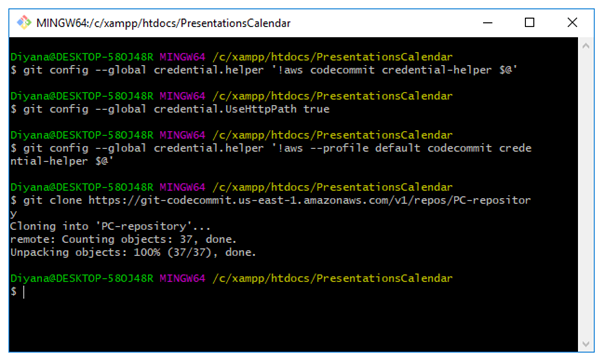
\includegraphics[scale=0.9]{clonerepo.png}
  \caption{Configuring and cloning the repository}
\end{figure}

\begin{figure}[h!]
\centering
    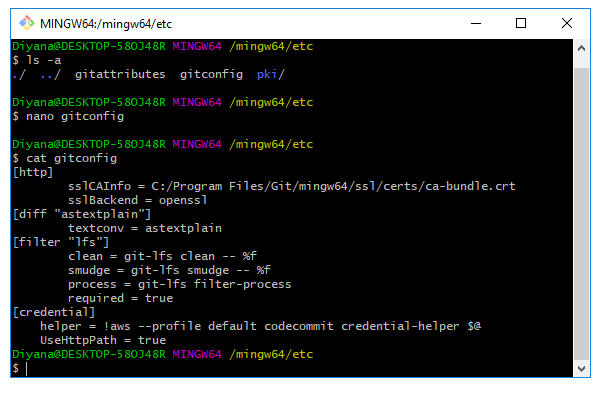
\includegraphics[scale=0.85]{localgitcredentials.png}
  \caption{Local folder Git -> [credential]}
\end{figure}

\begin{figure}[h!]
\centering
    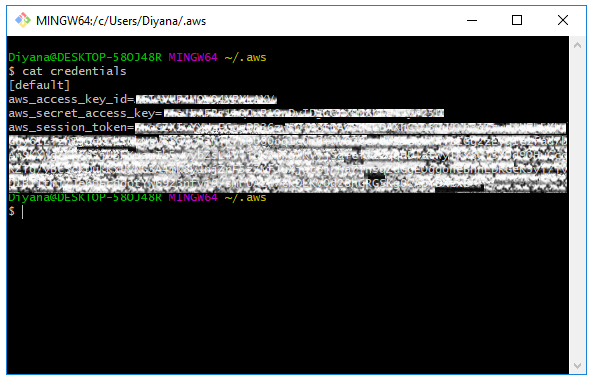
\includegraphics[scale=0.85]{localawscredentials.png}
  \caption{Local folder .aws -> [default]}
\end{figure}

\newpage

\noindent Извършва се локално клониране на целия проект в новосъздадена папка. За публикуването на проекта в cloud-а се използват стандартните git команди - commit и push.
\medskip

\noindent \textbf{ЗАБЕЛЕЖКА:} След изтичане на сесията от AWS educate, файлът credential от папка .aws трябва да се обнови с новите credential данни.

\subsection{AWS Elastic Compute Cloud}
\noindent Създава се EC2 инстанция от AWS Console. В стъпка 3: Configure Instance Details добавяме следните команди за стартиране на основни сървиси като Apache и допълнителни за него инструменти:
\medskip

\begin{figure}[h!]
\centering
    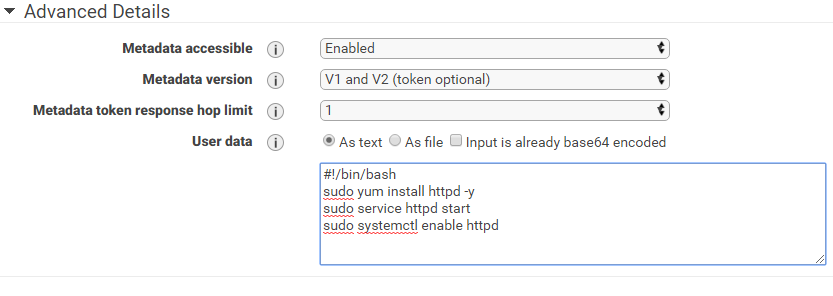
\includegraphics[scale=0.7]{createEC2.png}
  \caption{Advanced Details - EC2}
\end{figure}

\noindent При създаване на инстанцията се създава нова security група, в която добавяеследните правила: 
\begin{figure}[h!]
\centering
    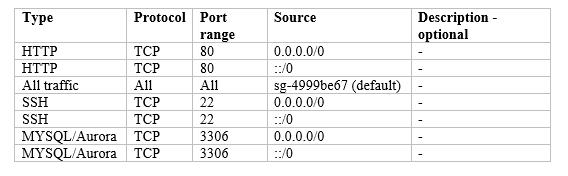
\includegraphics[scale=0.9]{sgrules.png}
  \caption{Security Group - Rules}
\end{figure}

\noindent \textbf{ЗАБЕЛЕЖКА:} Новосъздадена инстанция EC2 и RDS трябва да се намират в един и същи Virtual Private Cloud(VPC).
\medskip

\noindent След успешното създаване на инстанция EC2 се свързваме с нея. Аналогично на конфигурацията на локалната среда, конфигурираме файла gitconfig и файла credentials от папка .aws на машината в cloud-а. Това позволява клонирането на хранилището.

\begin{figure}[h!]
\centering
    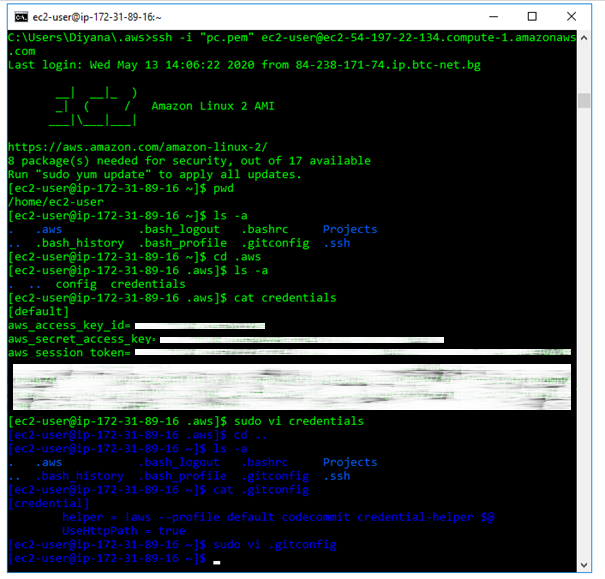
\includegraphics[scale=0.9]{publicCredentials.png}
  \caption{Configure EC2}
\end{figure}

\noindent За стартирането на проекта през Apache Server от cloud-а, всички файлове от проекта се преместват в директория \textbf{/var/www/html} с команда: 

\noindent \textbf{sudo cp -r “new-directory-name” /var/www/html}
\newpage

\begin{figure}[h!]
\centering
    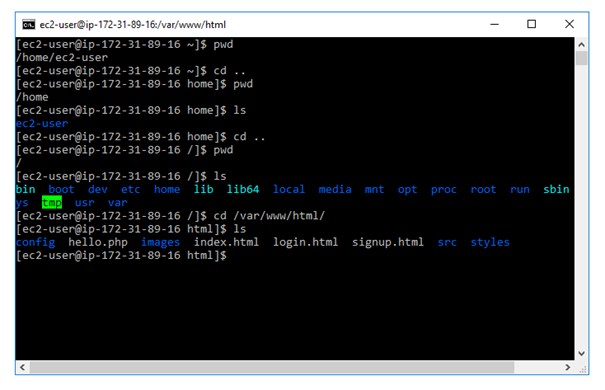
\includegraphics[scale=0.7]{projectOnApache.png}
  \caption{Project files that would be run by the Apache server}
\end{figure}

\noindent Добавя се допълнителнa конфигурация към файла \textbf{httpd.conf} на Apache, намиращ се в директория \textbf{/etc/httpd/conf}:

\begin{figure}[h!]
\centering
    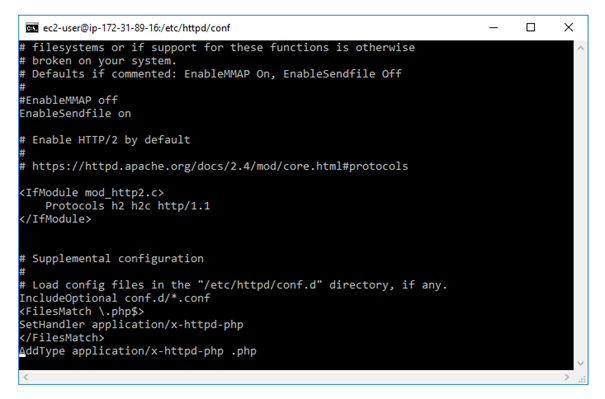
\includegraphics[scale=0.7]{confApache.png}
  \caption{Configure Apache}
\end{figure}

\newpage

\noindent Изпълняват се команди за допълнително конфигуриране и стартиране на PHP:

\noindent \textbf{sudo yum install php}

\noindent \textbf{sudo yum install php-pdo}

\noindent \textbf{sudo yum install php-pdo\_mysql}

\noindent \textbf{sudo service httpd restart}

\medskip

\noindentПриложението се достъпва чрез \textbf{Public DNS (IPv4)} или от \textbf{IPv4 Public IP} на създадената инстанция EC2.

\subsection{Amazon Machine Images - Backup}
\noindent AWS AMI е услуга, която позволява бързо и лесно да се създаде Backup на вече създадена и конфигуриране инстанция AWS EC2. В AMI предварително са конфигурирани Virtual Machine Image (VMI), съдържащ операционна система(ОС) нужен за създаване на инстанция. AWS предоставя и готови AMI-та, но предоставя и функционалност за създаване на ново. 
\medskip

\noindent За създаването на ново AMI от вече създадена AWS EC2 инстанция се изпълняват следните команди от AWS конзолата:
\medskip

\noindent \textbf{AWS services ->}

\noindent \textbf{EC2 ->}

\noindent \textbf{Instances ->}

\noindent \textbf{Click on instance ->}

\noindent \textbf{Actions ->}

\noindent \textbf{Create Image (Create AMI) ->}

\noindent \textbf{AMI is ready for use}

\newpage

\section{Кратко ръководство за потребителя}
\begin{figure}[h!]
\centering
    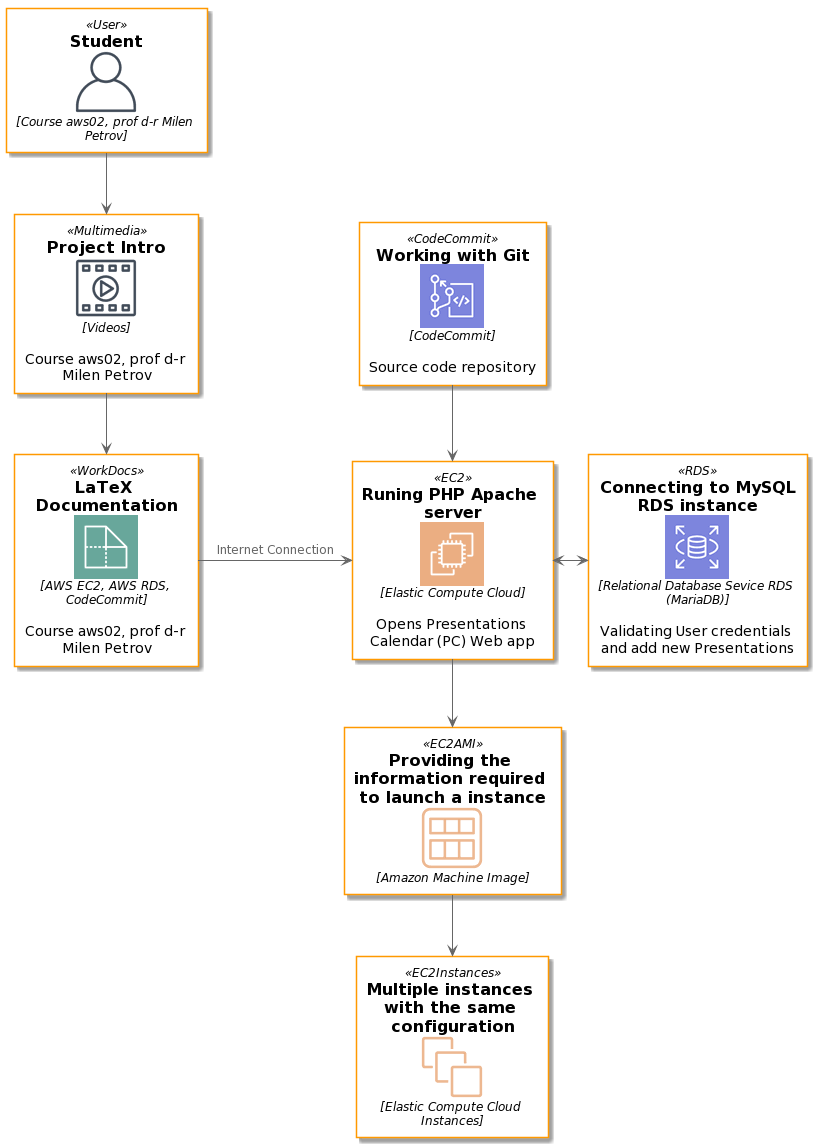
\includegraphics[scale=0.4]{diagram.png}
  \caption{Use Guide PlantUML Diagram}
\end{figure}

\newpage

\section{Примерни данни}
\begin{figure}[h!]
\centering
    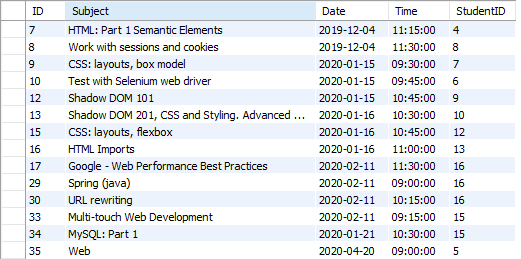
\includegraphics[scale=0.9]{presentations.png}
  \caption{Presentations data}
\end{figure}

\medskip

\begin{figure}[h!]
\centering
    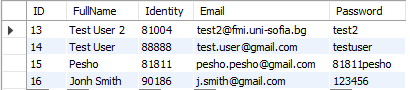
\includegraphics[scale=0.9]{students.png}
  \caption{Students data}
\end{figure}
 
\section{Описание на програмния код}
Кодът е разделен в няколко логически обособени части. 

\subsection{Презентационен слой}
\noindent HTML файловете в главната папка на проекта, файловете в папките css (файлове, отговарящи за стилизацията), imаges (изображения, използвани в страниците).
\medskip

\noindent HTML файловете са:
\begin{itemize}
    \item index.html - основна страница на Уеб приложението.
    
    \item login.html - страница за ВХОД на потребителя.
    
    \item signup.html - страница за Регистриране на нов потребител.
\end{itemize}

\subsection{Домейн слой}
\noindent PHP скриптове в подпапката src на главната папка на проекта:
\begin{itemize}
    \item addPresentation.php - скрипт, в който се извиква метод от db.php за добавяне на нов запис в таблицата calendardb.Presentations.
    
    \item authenticate.php - скрипт за удостоверяване на валидността на подадени данни при ВХОД на потребителя.
    
    \item calendar.php - визуализация на календара.
    
    \item day.php - визуализация на ден.
    
    \item db.php - имплементация на class DataBase, използващ се в целия проект и даващ достъп до база данни calendardb, с която работи уеб приложението.
    
    \item deletePresentation.php - скрипт, в който се извиква метод от db.php за премахване на запис от таблицата calendardb.Presentations.
    
    \item deletePresentationForm.php - форма за изтриване на записана презентация.
    
    \item generateCalendar.php - скрипт за динамично генериране на календар.
    
    \item generateDay.php - скрипт за динамично генериране на ден, съдържащ записи със запазени часове за представяне на презентации.
    
    \item home.php - начална страница на влезнали в системата потребители.
    
    \item logout.php - изход от системата.
    
    \item presentation.php - форма за записване на презентация.
    
    \item signup.php - скрипт за валидация и регистриране на нов потребител по въведени данни.
\end{itemize}

\newpage

\subsection{Структура на релационна база данни}
\noindentАрхитектурата на базата данни представлява:

\begin{figure}[h!]
\centering
    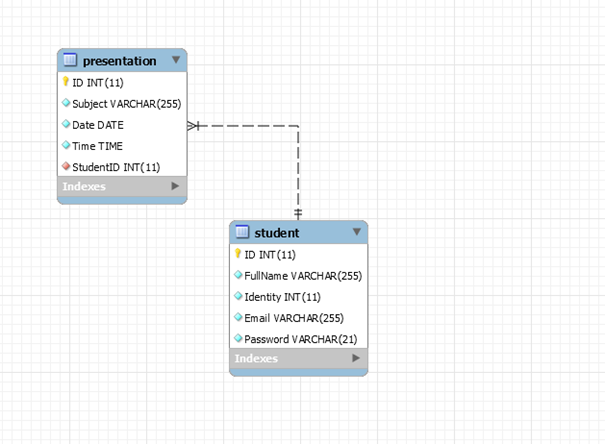
\includegraphics[scale=0.9]{db.png}
  \caption{Database - Architecture}
\end{figure}

\subsection{Обща картина на Уеб приложението}
\noindent При регистрация потребителят трябва да въведе свои лични данни – собствено и фамилно име, факултетен номер, имейл и парола. Системата проверява дали всички задължителни полета са попълнени, дали имейлът е валиден и дали факултетният номер, който е въвел студентът, е уникален. Ако не съществува вече регистриран потребител с подадения факултетен номер, то регистрацията на студента е успешна и той продължава към Вход в системата. 
\medskip

\noindent Вход в системата се осъществява с въвеждане на факултетен номер и парола на студента. След въвеждане на нужните данни, системата проверява дали тези данни са коректни – проверява дали за съответния факултетен номер съответства подадената парола.
\medskip

\noindent Ако Входът в системата е завършил с неуспех, тогава потребителят може да навигира до календара и да преглежда съдържанието, което е предоставено. Всякакви функционалности като добавяне и изтриване на запазена дата за представяне на презентация са неактивни за нерегистриран потребител. При липса на регистрация, всеки може да създаде такава, по всяко време. 
\medskip

\noindent Ако Регистрацията на студента е завършила с успех, то неговите данни биват записани в таблицата Student. Така по идентификационен номер в таблицата, при Вход се проверява валидността на факултетния номер и парола на студента. След безпроблемно влизане в системата, всеки потребител има възможност да навигира към календара със запазени дати за представяне на презентации, да запази своя дата или да изтрие запазена дата за презентация, само ако текущия потребител я е запазил.  Изтриването на чужди запазени дати е забранено за активните потребители. Всеки студент има достъп за триене само на своите презентации.
\medskip

\noindent При добавяне на нова презентация в таблицата Presentation се запазва запис за запазената дата. Така визуализирането на запазена дата за представяне на презентация става мигновенно.

\medskip


\section{Приноси на студента, ограничения и възможности за бъдещо развитие}
\noindent Представената функционалност в този документ е изработена изцяло от автора на този документ. Съществуват много възможности за бъдещо развитие като добавяне AWS CloudWatch и S3 при разширяване на функционалности на разгледания проект. 
\medskip

\section{Какво научих}
\noindent Благодарение на изпълнението на текущия проект за пръв път създадох цялостен web сайт, който да е качен в cloud пространството. При реализирането му не са използвани други framework и външни графични библиотеки. Запознах се с различни услуги, предоставени от AWS , MySql WorkBench при създаване на базата от данни, създаването на таблиците и съответно вкарването на разнообразните данни в тях. Подобрих познанията си в технологии като HTML, CSS, MySQL, PHP и Apache.

\section{Списък с фигури}
%\listoftables

\listoffigures

\section{Използвани източници}
\noindent\href{https://aws.amazon.com/ec2/}{[1] AWS Elastic Compute Cloud}

\noindent\href{https://aws.amazon.com/rds/}{[2] AWS Relational Database Service}

\noindent\href{https://aws.amazon.com/codecommit/}{[3] CodeCommit}

\noindent\href{https://learn.fmi.uni-sofia.bg/course/view.php?id=6143}{[4] AWS FMI Course}

\noindent\href{https://docs.aws.amazon.com/codecommit/latest/userguide/setting-up-https-unixes.html}{[5] Setup the Credential Helper on Git}

\noindent\href{https://docs.aws.amazon.com/index.html}{[6] AWS Documentation}

\end{document}
